%
% The first command in your LaTeX source must be the \documentclass command.
\documentclass[sigconf]{acmart}
\usepackage[ruled,vlined]{algorithm2e}

%
% \BibTeX command to typeset BibTeX logo in the docs
\AtBeginDocument{%
  \providecommand\BibTeX{{%
    \normalfont B\kern-0.5em{\scshape i\kern-0.25em b}\kern-0.8em\TeX}}}

% Rights management information. 
% This information is sent to you when you complete the rights form.
% These commands have SAMPLE values in them; it is your responsibility as an author to replace
% the commands and values with those provided to you when you complete the rights form.
%
% These commands are for a PROCEEDINGS abstract or paper.
\copyrightyear{2018}
\acmYear{2018}
\setcopyright{acmlicensed}
\acmConference[Woodstock '18]{Woodstock '18: ACM Symposium on Neural Gaze Detection}{June 03--05, 2018}{Woodstock, NY}
\acmBooktitle{Woodstock '18: ACM Symposium on Neural Gaze Detection, June 03--05, 2018, Woodstock, NY}
\acmPrice{15.00}
\acmDOI{10.1145/1122445.1122456}
\acmISBN{978-1-4503-9999-9/18/06}

%
% These commands are for a JOURNAL article.
%\setcopyright{acmcopyright}
%\acmJournal{TOG}
%\acmYear{2018}\acmVolume{37}\acmNumber{4}\acmArticle{111}\acmMonth{8}
%\acmDOI{10.1145/1122445.1122456}

%
% Submission ID. 
% Use this when submitting an article to a sponsored event. You'll receive a unique submission ID from the organizers
% of the event, and this ID should be used as the parameter to this command.
%\acmSubmissionID{123-A56-BU3}

%
% The majority of ACM publications use numbered citations and references. If you are preparing content for an event
% sponsored by ACM SIGGRAPH, you must use the "author year" style of citations and references. Uncommenting
% the next command will enable that style.
%\citestyle{acmauthoryear}

%
% end of the preamble, start of the body of the document source.
\begin{document}

%
% The "title" command has an optional parameter, allowing the author to define a "short title" to be used in page headers.
\title{Real-Time Eye Tracking System with Parallel Image Processing}

%
% The "author" command and its associated commands are used to define the authors and their affiliations.
% Of note is the shared affiliation of the first two authors, and the "authornote" and "authornotemark" commands
% used to denote shared contribution to the research.
\author{Bo-Chun Chen}
\email{coslate@media.ee.ntu.edu.tw}
\affiliation{%
  \institution{Credit Program on Colleges of Electrical and Computer Engineering and Computer Science \\The Center for Continuing Education and Training \\ National Chiao Tung University}
  \streetaddress{No. 90, Jinshan 11th St}
  \city{HsinChu}
  \country{Taiwan}}



% By default, the full list of authors will be used in the page headers. Often, this list is too long, and will overlap
% other information printed in the page headers. This command allows the author to define a more concise list
% of authors' names for this purpose.
\renewcommand{\shortauthors}{Bo-Chun Chen}

%
% The abstract is a short summary of the work to be presented in the article.
\begin{abstract}
Eye tracking system has high potential as a natural user interface device;
however, the mainstream systems are designed with infrared illumination, which may be harmful for human eyes.
In this paper, a real-time eye tracking system is proposed without Infrared Illumination.
To deal with various lighting conditions and reflections on the iris, the proposed system is based on a continuously updated color model for robust iris detection. Moreover, the proposed algorithm employs both the simplified and the original eye images to achieve the balance between robustness and accuracy. Multiple parallelism techniques including TBB, CUDA, POSIX and OpenMP can be used to speedup the process. The Experimental results are targeted to show that the proposed system can capture the movement of user's eye with standard deviation smaller than 10 pixels compared to ground truth, and the processing speed can be up to 30fps.
\end{abstract}


%
% Keywords. The author(s) should pick words that accurately describe the work being
% presented. Separate the keywords with commas.
\keywords{Eye tracking, eye localization, eye movement, Parallel Programming, POSIX, CUDA, OpenMP, TBB}

%
% A "teaser" image appears between the author and affiliation information and the body 
% of the document, and typically spans the page. 
%\begin{teaserfigure}
%  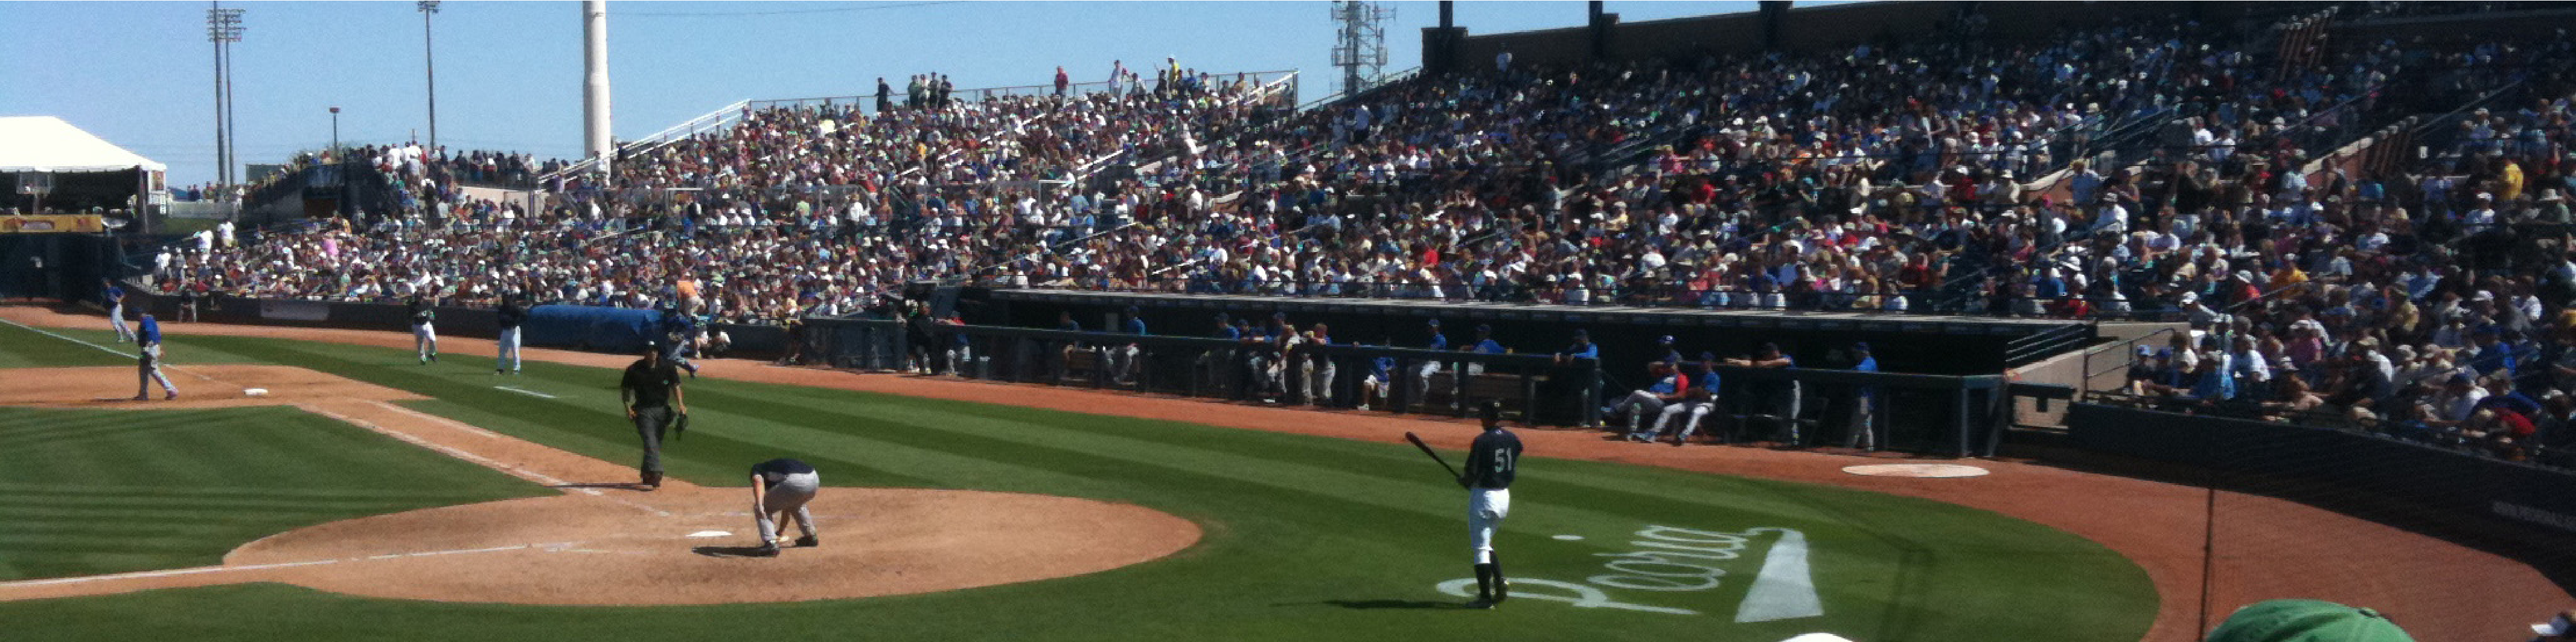
\includegraphics[width=\textwidth]{sampleteaser}
%  \caption{Seattle Mariners at Spring Training, 2010.}
%  \Description{Enjoying the baseball game from the third-base seats. Ichiro Suzuki preparing to bat.}
%  \label{fig:teaser}
%\end{teaserfigure}

%
% This command processes the author and affiliation and title information and builds
% the first part of the formatted document.
\maketitle

\section{Introduction}
\label{sec:intro}
Eye tracking tracking is a highly potential technique for natural user interface, especially for wearable devices. Most existing wearable eye trackers employ infrared illumination to achieve robust performance
by stable lighting conditions with infrared light sources close to the eyes. Since infrared light is invisible, it does not distract users, and the pupil becomes obvious and easy to detect under infrared illumination.  However, infrared light sources illuminating eyes in such a close distance may cause harms to eyes. Radiation in the near infrared light is the most hazardous and is transmitted by the optical components of eyes \cite{seeber2007light}. It has higher transmission rate and lower absorption rate than visible light, and near infrared light can eventually reaches the retina while visible light is always absorbed by cornea \cite{Teaching}. If one is overexposed to infrared light, it may cause the thermal retina burn \cite{doi:10.1080/713820456}. 

In this work, we propose a new solution with parallel programming for eye tracking system without infrared illumination. To deal with the variation of uncontrolled lighting conditions and maintain the accuracy as well,
several strategies are proposed. First, an iris color model is utilized for robust iris detection, which is continuously updated to address various lighting conditions. Second, the proposed system employs a simplified and original eye images at the same time as a kind of multi-scale algorithm. The simplified image is employed to detect coarse seed point and mask impossible feature points. Third, a modified Starburst algorithm is proposed with an iris mask for eye images without infrared illumination. The first and second part includes several filter and morphological operation, which can be speedup by parallelism, while the third part is a sequential procedure which has limited parallelism.

\section{Statement of the problem}
Most application of an eye tracking system is to map information of an eye to a gaze point, which can be used to build attention model or some user interface. The features of an eye must be stable and same when we gaze at same point, different when we gaze at different gaze point, that is, to have high intra-class similarity and low inter-class similarity. Research in the past detect the center of pupil as the feature of an eye according to the fact that infrared light can make the image of pupil clear, noise-free and thus very easy to detect\cite{5068882}\cite{Morimoto2000331} as shown in Fig.~\ref{fig:infrared}(a). However, without infrared illumination, the most prominent feature of an eye is the limbus, which is the boundary of sclera and iris. Fig.~\ref{fig:infrared}(b) shows the eye image without infrared illumination. Due to the reflection in the iris, it is hard to detect the pupil. The only choice is to detect the cornea center because of being concentric with pupil. Unfortunately, the iris is always cropped by eyelids and corners of the eye. If one wants to detect the entire iris region, the best way to do is to open his/her eyes as much as possible, and it would be too tired to use a system. Instead, we only need a stable and distinguishable point to represent the position of an eye. So the problem is to find a way to represent the center of iris with high intra-class similarity and low inter-class similarity as our feature of an eye.

\begin{figure}
\centering
\begin{tabular}{cc}
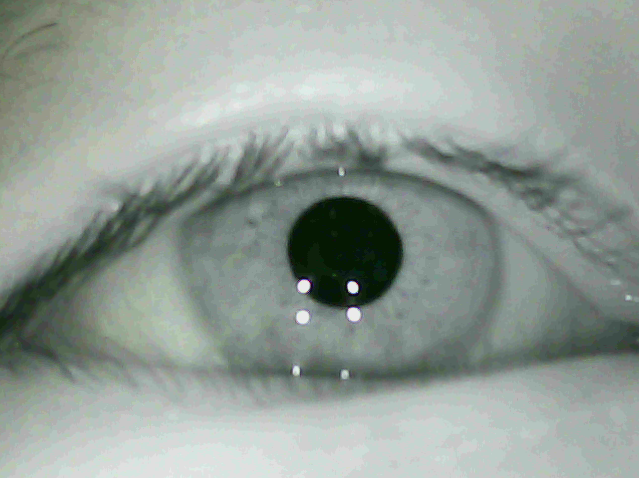
\includegraphics[width=4cm]{../Fig/infrared_spectrum.png} &
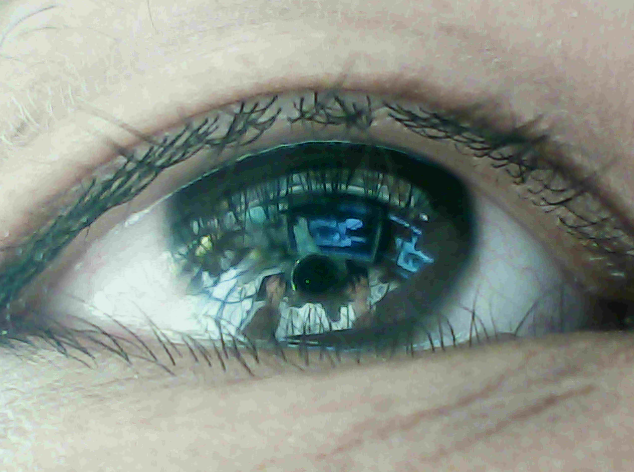
\includegraphics[width=4cm]{../Fig/visible_spectrum.png} \\
(a) & (b)
\end{tabular}
\caption{(a) With infrared illumination. (b) Without infrared illumination.}
\label{fig:infrared}
\end{figure}

\section{Proposed approaches}
\begin{figure}
\begin{minipage}[b]{1.0\linewidth}
  \centering
%  \centerline{\includegraphics[width=8.2cm]{../Fig/Overview_Algorithm_highlight.png}}
  \centerline{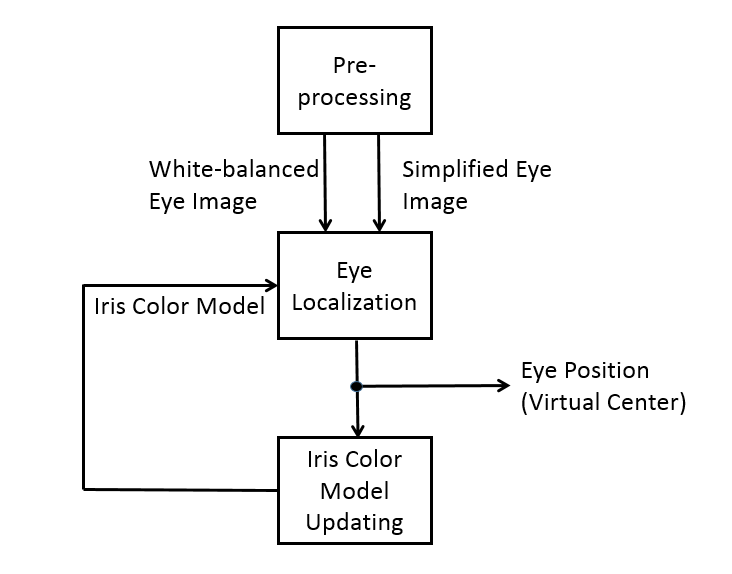
\includegraphics[scale=0.6]{../Fig/System_Overview.png}}
%  \vspace{2.0cm}
\end{minipage}
\caption{System overview}
\label{fig:System overview}
\end{figure}

%========================================
Fig.~\ref{fig:System overview} shows the overview of the whole system.
The input of the system is an eye image. Different from the eye images acquired under infrared illumination, the eye images under normal lighting conditions usually contain noise from lighting condition variation and reflection of environment, as shown in Fig.~\ref{fig:preprocessing}(a). Therefore, the first step is image pre-processing, which aims to filter out the distortion and noise of input eye image. Since the color information is critical to the whole system, we correct the color with automatic white balance to generate image $I_E$. Moreover, a simplified gray-scale eye image $\hat{I_E}$ is also generated with histogram equalization, morphological gray opening operation, and Gaussian blurring operation to reduce the reflection inside the iris, as shown in Fig.~\ref{fig:preprocessing}(b). As mentioned in Section~\ref{sec:intro}, both these two images are employed in the eye localization as a kind multi-scale processing: the simplified image is used to generate rough detection and masking information robustly, while the white-balanced image is utilized to generated accurate eye location accordingly. An iris color modeled is also maintained in this system to address various lighting conditions. While the iris color model keeps improving itself, the result of eye position, the virtual center, is also getting more accurate, and vice versa. The details of the algorithm are described in the following subsections.


\begin{figure}
\centering
\begin{tabular}{cc}
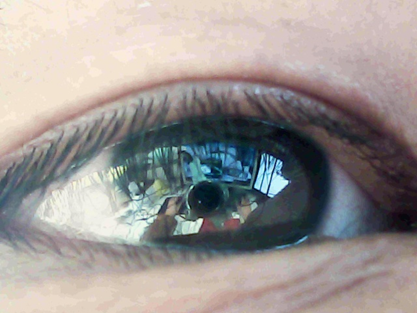
\includegraphics[width=4cm]{../Figures/visible_eye.png} &
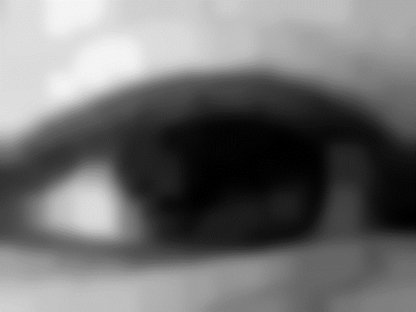
\includegraphics[width=4cm]{../Figures/simplified.png} \\
(a) & (b)
\end{tabular}
\caption{(a) White-balanced eye image $I_E$. (b) Simplified eye image $\hat{I_E}$.}
\label{fig:preprocessing}
\end{figure}


\subsection{Eye Localization}

The purpose of eye localization is to find a stable feature that can represent the location of an eye
with high intra-class similarity and low inter-class similarity.
We define the stable feature point as a ``virtual center.''
The virtual center in our system is not the location of pupil
but is the center of the region surrounded by the feature points at eyelids and left/right sides of limbus.
%We find out that the eyelids can be used with left and right sides of limbus to define the virtual center.
The method of feature point detection is based on Starburst algorithm \cite{Li:2005:SHA:1099539.1099986},
which is originally invented to detect the boundary of one's pupil under infrared illumination.
Because the pupil is invisible under visible light, it is proposed to change the target to limbus and eyelids.

In order to make Starburst algorithm robust enough to detect feature points under visible light
and have the ability to adapt to variant lighting conditions, two distinct features are developed and added.
The first added feature is the automatic seed point finding algorithm.
In the original Starburst algorithm, the seed point is picked as the center point of a frame.
In order to automatically find the seed point with illumination invariant property,
a color model with 2D h-s (hue-saturation) histogram is constructed for the iris region.
During initialization, the rough iris region is estimated by calculating the moment center of the binarized version of $\hat{I_E}$
followed by a region growing process.
Within the rough iris region, the h-s histogram of $I_E$ is calculated as the initial iris color model.
After the iris color model is established, for an input eye image $I_E$, the back projection of the iris color model is derived by replacing the value of each pixel $(i,j)$ with the corresponding normalized bin value in the h-s histogram. That is,
\begin{equation}
I_{BP}(i,j) = H(h_{i,j}, s_{i,j}),
\end{equation}
where the higher value means that the corresponding position has a higher probability to be a part of the iris region, as shown in Fig.~\ref{fig:BPF}(b).
The seed point is then generated with binarization and moment center calculation.
In the following frames, in order to deal with various lighting conditions, the iris color is updated every specified number of frames.
To do so, a rough iris mask $M_{RI}$ is generated by finding the convex hull of the binarized $\hat{I_E}$, as shown in Fig.~\ref{fig:BPF}(c).
A new h-s histogram of $I_E$ is calculated inside the mask $M_{RI}$.
The back projection $I_{BP}$ is then generated as well as an index called iris ratio, which is defined as.
 \begin{equation}
\mbox{Iris Ratio} = \frac{\eta}{\sigma},
\end{equation}
where $\eta$ means the sum of probability of iris point inside the mask $M_{RI}$,
and $\sigma$ means the sum of probability of iris point outside the mask.
Greater iris ratio comes a more representative model,
and we discard those 2D h-s histogram models with low iris ratio.


The second feature added is the iris mask 
that is used to mask out the reflection in iris region and other impossible feature points to enhance Starburst algorithm.
As shown in Figs.~\ref{fig:ova}(a)--(c), the iris region is estimated with projections of the simplified image $\hat{I_E}$.
Eyelid fitting is then done by modeling the upper and lower eyelids as two parabolas.
With the simplified image $\hat{I_E}$, the valley-peak field, Fig.~\ref{fig:ova}(f),
is generated by calculating the convex-hull of the extracted iris rectangle with the biggest circle in it, as shown in Fig.~\ref{fig:ova}(e),
and the pixels with large horizontal gradient but low vertical gradient, as shown in Fig.~\ref{fig:ova}(d).
We then use the eyelid feature points outside the valley-peak field to fit upward and downward parabola functions, as shown in Fig.~\ref{fig:ova}(g).
The intersection of the region inside the eyelid and the estimated iris region as Fig.~\ref{fig:ova}{c} forms the iris mask $M_I$ for our modified Starburst algorithm described as Algorithm~\ref{alg:starburst}, and the feature points are then generated as shown in Fig.~\ref{fig:ova}(h), where the navy blue and light blue feature points represent the inliers of upper and lower eyelid parabolas individually, and green feature points represent the limbus feature points detected by our modified Starburst algorithm~\ref{alg:starburst}. All the feature points will be used to form convex hull as shown in Figs.~\ref{fig:ova}(i)--(j), and this is how the accurate iris mask $M_{AI}$ generated.
Finally, the location of the virtual center $(X_e, Y_e)$ is derived from the moment center of the inverted version of $\hat{I_E}$ masked by $M_{AI}$, as shown in Figs.~\ref{fig:ova}(k)--(l) and the following equations.
\begin{align}
m_{i, j} &= \sum_{x,y}{(255-\hat{I_E}) \cdot M_{AI} \cdot x^i y^j},\\
X_e &= m_{1,0}/m_{0,0}, Y_e = m_{0,1}/m_{0,0}
\end{align}


\begin{figure}[t]
\begin{minipage}[b]{0.32\linewidth}
  \centering
  \centerline{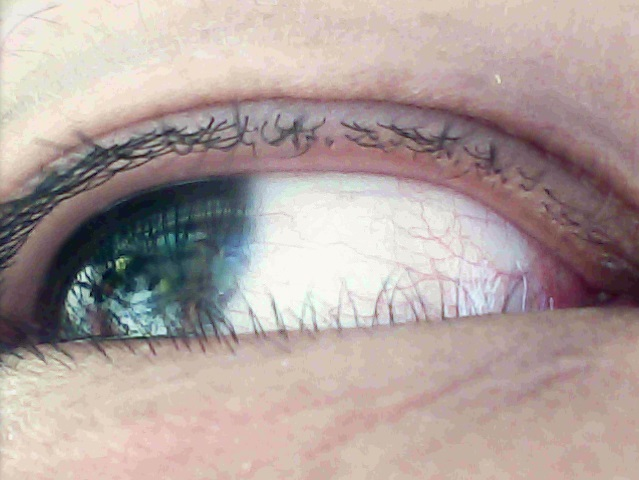
\includegraphics[width=2.5cm]{../Fig/IrisModelUpdating/ImageForValidTesting.jpg}}
%  \vspace{1.5cm}
  \centerline{(a)}\medskip
\end{minipage}
\hfill
\begin{minipage}[b]{0.32\linewidth}
  \centering
  \centerline{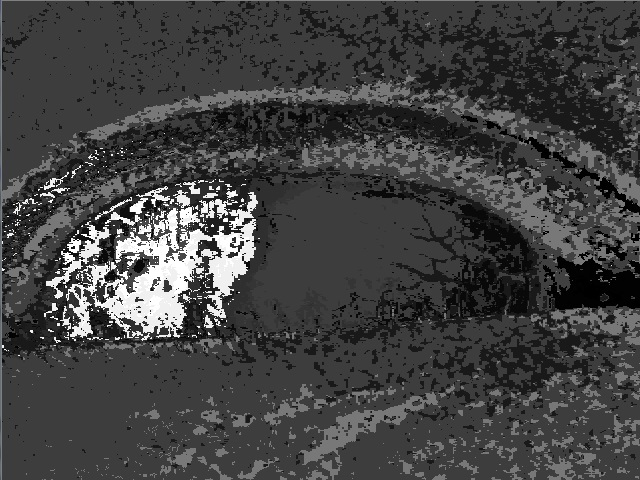
\includegraphics[width=2.5cm]{../Fig/IrisModelUpdating/BackProjection.jpg}}
%  \vspace{1.5cm}
  \centerline{(b)}\medskip
\end{minipage}
%
\hfill
\begin{minipage}[b]{0.32\linewidth}
  \centering
  \centerline{
\includegraphics[width=2.5cm]{../Fig/IrisModelUpdating/IrisRegion.jpg}}
%  \vspace{1.5cm}
  \centerline{(c)}\medskip
\end{minipage}
%
\caption{Hue-saturation histogram model refreshment (a) Input eye image. (b) Back projection $I_{BP}$.
		(c) Rough iris mask $M_{RI}$.}
\label{fig:BPF}
\end{figure}


\begin{figure}[t]
\begin{minipage}[b]{.32\linewidth}
  \centering
  \centerline{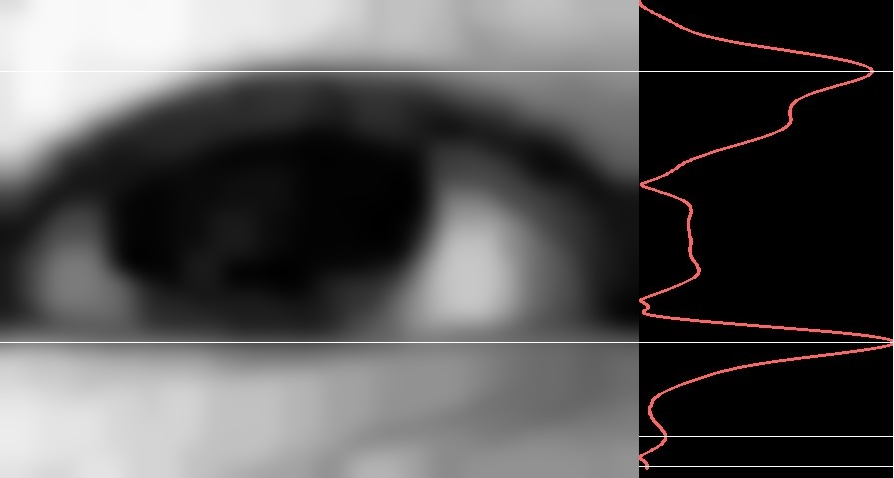
\includegraphics[width=3cm]{../Fig/IrisRegionExtraction_GPF/Deriv_hy_result.png}}
%  \vspace{1.5cm}
  \centerline{(a)}\medskip
\end{minipage}
\hfill
\begin{minipage}[b]{0.32\linewidth}
  \centering
  \centerline{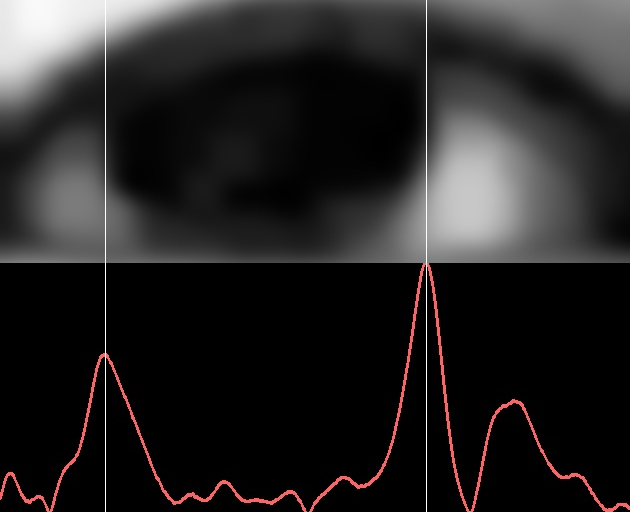
\includegraphics[width=2.5cm]{../Fig/IrisRegionExtraction_GPF/Deriv_vx_result.png}}
%  \vspace{1.5cm}
  \centerline{(b)}\medskip
\end{minipage}
%
\hfill
\begin{minipage}[b]{0.32\linewidth}
  \centering
  \centerline{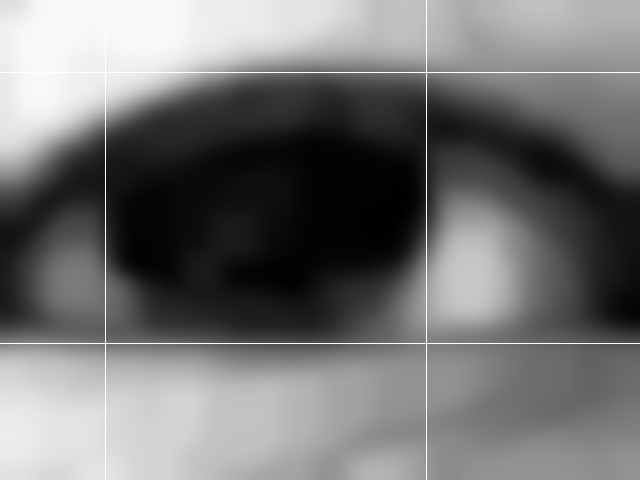
\includegraphics[width=2.5cm]{../Fig/IrisRegionExtraction_GPF/Resulted_irisRegionExtraction.jpg}}
%  \vspace{1.5cm}
  \centerline{(c)}\medskip
\end{minipage}
%
\vfill
\begin{minipage}[b]{0.32\linewidth}
  \centering
  \centerline{
\includegraphics[width=2.5cm]{../Fig/EyelidDetection/RefinedGradX_EyeRegion.jpg}}
%  \vspace{1.5cm}
  \centerline{(d)}\medskip
\end{minipage}
\hfill
\begin{minipage}[b]{0.32\linewidth}
  \centering
  \centerline{
\includegraphics[width=2.5cm]{../Fig/EyelidDetection/RefinedGradX_EyeRegion_Plus_IrisCenter.jpg}}
%  \vspace{1.5cm}
  \centerline{(e)}\medskip
\end{minipage}
\hfill
\begin{minipage}[b]{0.32\linewidth}
  \centering
  \centerline{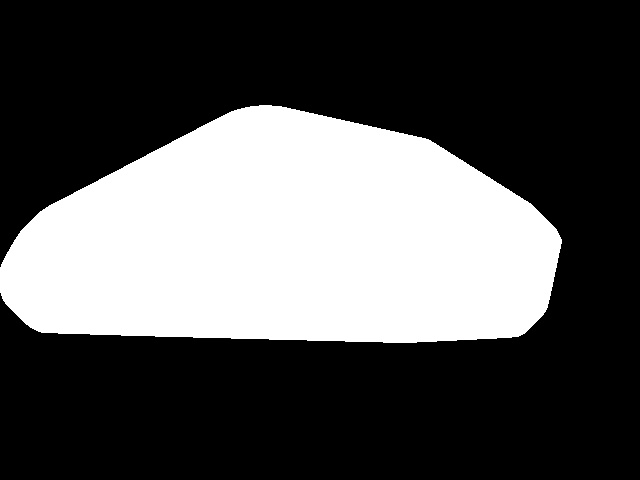
\includegraphics[width=2.5cm]{../Fig/EyelidDetection/ValleyPeakField.jpg}}
%  \vspace{1.5cm}
  \centerline{(f)}\medskip
\end{minipage}
\hfill
\begin{minipage}[b]{0.32\linewidth}
  \centering
  \centerline{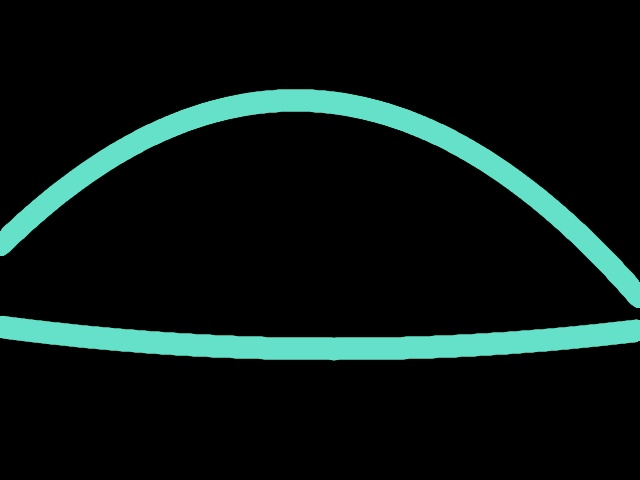
\includegraphics[width=2.5cm]{../Fig/EyelidDetection/Eyelid_Result.jpg}}
%  \vspace{1.5cm}
  \centerline{(g)}\medskip
\end{minipage}
\hfill
\begin{minipage}[b]{0.32\linewidth}
  \centering
  \centerline{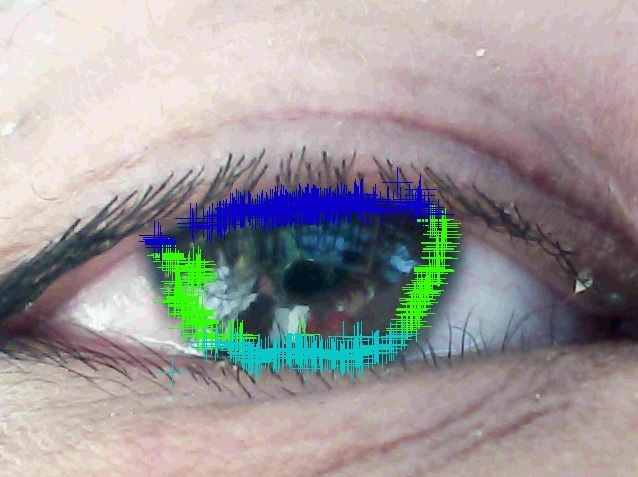
\includegraphics[width=2.5cm]{../Fig/ClipFeaturePts/ClipFeaturePointsDisp.jpg}}
%  \vspace{1.5cm}
  \centerline{(h)}\medskip
\end{minipage}
\hfill
\begin{minipage}[b]{0.32\linewidth}
  \centering
  \centerline{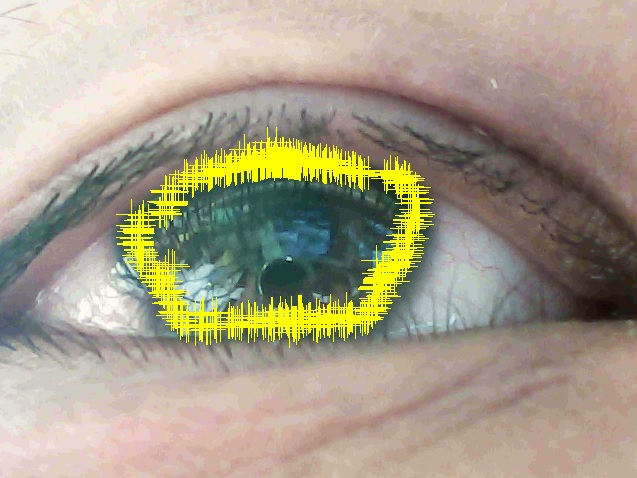
\includegraphics[width=2.5cm]{../Fig/ExactIrisCenter/RefinedFeaturePts.jpg}}
%  \vspace{1.5cm}
  \centerline{(i)}\medskip
\end{minipage}

\begin{minipage}[b]{0.32\linewidth}
  \centering
  \centerline{
\includegraphics[width=2.5cm]{../Fig/ExactIrisCenter/FeaturePoints_LimbusFtPtsConvexHull.jpg}}
%  \vspace{1.5cm}
  \centerline{(j)}\medskip
\end{minipage}
\hfill
\begin{minipage}[b]{0.32\linewidth}
  \centering
  \centerline{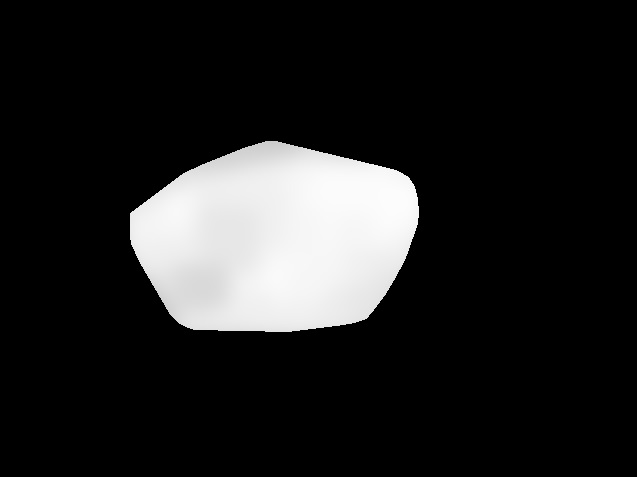
\includegraphics[width=2.5cm]{../Fig/ExactIrisCenter/MomentCenterByGrayLevel.jpg}}
%  \vspace{1.5cm}
  \centerline{(k)}\medskip
\end{minipage}
\hfill
\begin{minipage}[b]{0.34\linewidth}
  \centering
  \centerline{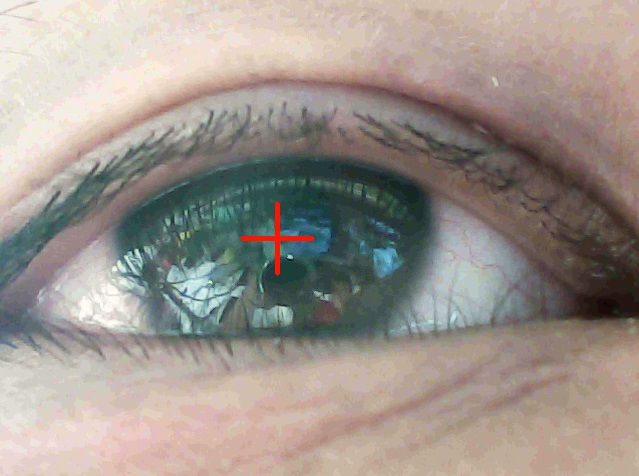
\includegraphics[width=2.5cm]{../Fig/ExactIrisCenter/EyePosition_CenterResult.jpg}}
%  \vspace{1.5cm}
  \centerline{(l)}\medskip
\end{minipage}


\caption{(a) Input image and the horizontal projection. (b) Input image and the vertical projection. (c) Extracted iris rectangle. (d) High x-directed gradient but low y-directed gradient pixels. (e) Fig.~\ref{fig:ova}(d) plus extracted biggest circle. (f) Valley-Peak field. (g) Fitted parabolas of eyelids. (h) Detected inliers of both parabolas of eyelids and limbus feature points. (i) All the detected feature points. (j) Accurate iris mask $M_{AI}$. (k) Inverted iris masked simplifed eye image. (l) Virtual center.}
\label{fig:ova}
\end{figure}


\begin{algorithm}[t]
  \KwIn{Preprocessed eye image $I_E$ and iris mask $M_{I}$}
  \KwOut{Feature points surrounding iris}
  initialization;\\
  \While{seed point does not converge}{
    clear F, the set of final feature points\;
    Stage1:\\
    Emit rays radially from the seed point with angle ranging in $[0,2\pi]$\;
    \For{Each ray}{
      Move extendedly along the ray from the seed point\;
      Calculate derivation of intensity at each pixel\;
      \If{Outside the iris mask $\wedge$ derivation $>$ 0} 
      {
        Push feature point to F\;
      }
    }
    Stage2:\\
    \For{Each candidate feature point detected in Stage 1}{
      Estimate the angle of the line from the feature point to the seed point, called $Ang_{fs}$\;
      Emit rays from the feature point back to the seed points with angle ranging in $[Ang_{fs} - \pi/12 , Ang_{fs} + \pi/12]$\;
      \For{Each ray}{
        Move backward along the ray from the the feature point\;
        Calculate derivation of intensity at each pixel\;
        \If{Outside the iris mask $\wedge$ derivation $>$ 0}{
          Push feature point to F\;
        }
      }

    }
   
    Seed point $\leftarrow$ Geometry center of feature points\;
  }
\caption{Modified Starburst Algorithm}
\label{alg:starburst}.
\end{algorithm}

\subsection{Parallelism}
The parallelism of the eye tracking system can be divided into two main categories: 'parallel in block' and 'parallel in channel' as shown in Fig.~\ref{fig:parallelism_tiling}(a)--(b).

If the operation is identical with each pixel, such as Gaussian filtering, RGB to gray convertion and morphological operation in the pre-processing block, iris color model back projection and binary operation in the iris color model updating block, masking and simplified projection in the eye localization block, then we can divide one image frame into several blocks and use 'parallel in block' technique as shown in Fig.~\ref{fig:parallelism_tiling}(a). The number of block can be defined by the number of CPU or GPU cores in one's computer, for example, 4 CPU cores in Fig.~\ref{fig:parallelism_tiling}(a). Each block can be processed through a sequence of image processing pipeline individually until the next image processing stage needs information from other blocks. The longer length of the sequence may produce better efficiency since the fork-join of threads will take some overhead.

If we are dealing with color image frames, which have multiple channels, then we can further apply 'parallel in channel' technique if the operation to all channels are identical, such as auto-white-balencing in the pre-processing block and RGB to HSV convertion in the iris color model updating block. As shown in Fig.~\ref{fig:parallelism_tiling}(b) for example, three channels can be propagated through image processing pipeline individually until the next image processing stage needs information from other channels. Besides, in one channel, we can further deploy 'parallel in block' if the operation to all pixels are identical, for example, the HSV histogram calculation in the iris color model updating block.

\begin{figure}[t]
\begin{minipage}[b]{0.8\linewidth}
  \centering
  \centerline{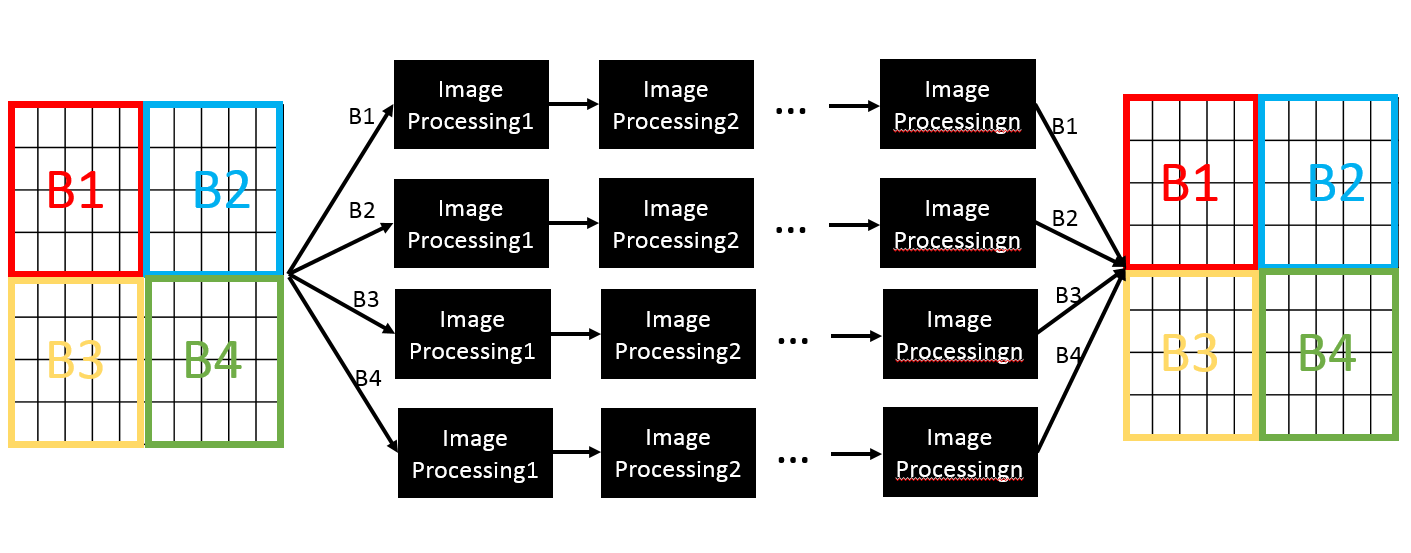
\includegraphics[width=8cm]{../Fig/Parallel_Tiling.png}}
%  \vspace{1.5cm}
  \centerline{(a)}\medskip
\end{minipage}
%
\vfill
\begin{minipage}[b]{0.8\linewidth}
  \centering
  \centerline{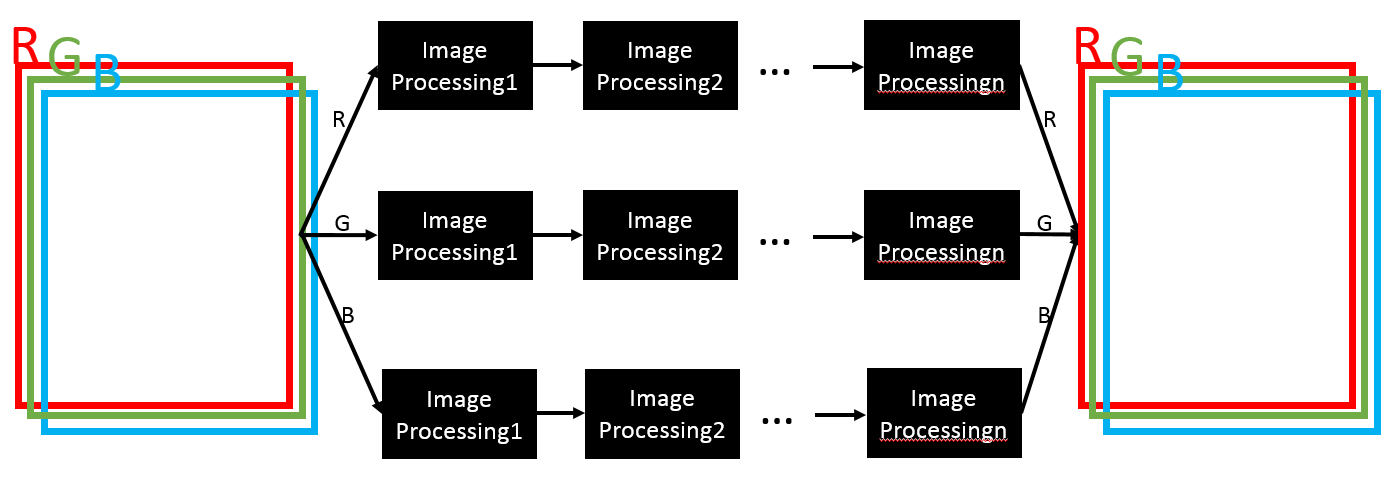
\includegraphics[width=8cm]{../Fig/Parallel_Tiling_Color.png}}
%  \vspace{1.5cm}
  \centerline{(b)}\medskip
\end{minipage}
\caption{(a) Parallel in block. (b) Parallel in channel}
\label{fig:parallelism_tiling}
\end{figure}


\section{Language selection}
C++ with OpenCV library is the programming language chosen to implement in this work according to its speed, efficiency and multiple parallel-library supporting. OpenMP and TBB with OpenCV will be used to fork and join parallel tasks though CPU cores. CUDA with OpenCV will also be considered to parallelize some tasks on GPU cores. C++ along with OpenCV will also be applied to implement some I/O and GUI implementation.

\section{Related work}
%According to having infrared illumination or not, the method can be classified into two categories: limbus detection, and pupil detection. It is because that under infrared illumination, the boundary between pupil and cornea is very distinguishable as shown in Fig.~\ref{fig:infrared}(a). However, when being illuminated without infrared light, pupil is not visible under most of the situations as Fig.~\ref{fig:infrared}(b). The only noteworthy feature is the boundary between cornea and sclera, in other words, the limbus. 

Ryan et al.\cite{Ryan:2008:LSW:1344471.1344487} switches between limbus detection and pupil detection due to the lightness of environment. They use pupil detection in bright light, and use limbus detection in dim light. Starburst\cite{Li:2005:SHA:1099539.1099986} algorithm and ellipse fitting with RANSAC technique are used to find the pupil and cornea in their work. Ebisawa\cite{5068882} uses dark and bright pupil difference technique to detect pupil. The work is shown in Fig.~\ref{fig:Difference of bright and dark pupil technique}. Bright pupil image is generated by turning on the ring-like Infrared light sources attached around the aperture of a camera. Dark pupil image is generated by turning on other ring-like infrared light sources attached away from the aperture. After getting the difference image, setting a threshold and extract the connected component will give a result of pupil contour\cite{Morimoto2000331}. The accuracy of this kind of work is in the range of 5-20 pixels.

\begin{figure}
\begin{minipage}[b]{1.0\linewidth}
  \centering
  \centerline{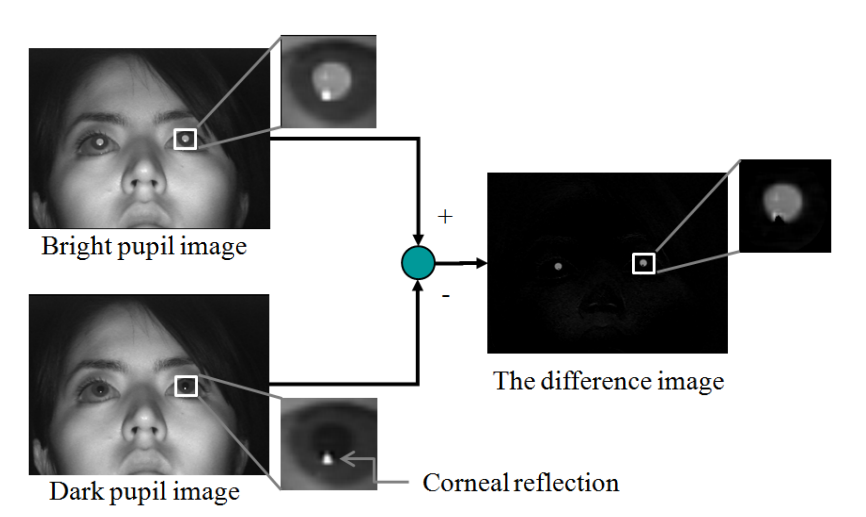
\includegraphics[scale=0.3]{../Fig/Dark_bright_pupil_difference_technique.png}}
\end{minipage}
\caption{Difference of bright and dark pupil technique\cite{5068882}}
\label{fig:Difference of bright and dark pupil technique}
\end{figure}


\section{Statement of expected results}
Current system is implemented in Visual C++ and OpenCV library \cite{opencv_library} on a personal computer with a 4.0-GHz CPU and 24-GB RAM. The size of the monitor is 22 inches and the aspect ratio is 16:10$ \left(\;47.39\times29.61\; cm^2\right)$.
The resolution of an eye image is 640$\times$480, and the resolution of the screen is 1680$\times$1050.
The distance between the user and the monitor is 50c.m away in front of the monitor, which makes my field of view limited to the size of the monitor.
The visual angle ranges horizontally in $\left[-25.35 , 25.35\right]$ $\left(degree\right)$ and vertically in $\left[-16.49 , 16.49\right]$ $\left(degree\right)$. 
The experiments conducted with the current system shows that the processing speed of the whole system is 10--11fps, and the average accuracy is about 10 pixels, which is comparable to those systems using multiple infrared light sources and multiple cameras.
After being parallelized, it is expected to be 1.6 times speedup under 2 CPU cores, which is 16fps, and 3.2 times speedup under 4 CPU cores, which is around 30fps while the accuracy should remain almost same, that is, 10 pixels.


\section{A timetable}
The schedule is described as Table \ref{tab:schedule}.

\begin{table}[t]
\centering
\caption{Timetable}
\label{tab:schedule}
\begin{tabular}{ccc}
\hline
\hline
Item                & Schedule     & Comment\\
\hline
Experiment environment & 4/15-4/22  & error format(mean+std).     \\
Profiling              & 4/23-4/29  & cost of time. \\
Implementation         & 4/30-5/27  & OpenMP+TBB+CUDA \\
Experiments            & 5/28-6/10  & OpenMP+TBB+CUDA \\
Presentation slides    & 6/11-6/24  & presentation slides ready \\
\hline
\hline
\end{tabular}
\end{table}


%
% The next two lines define the bibliography style to be used, and the bibliography file.
\bibliographystyle{ACM-Reference-Format}
\bibliography{sample-base}


\end{document}
